\section{时序图查询语言}
RDF的标准查询语言SPARQL并没有与时序相关的语法,所以需要在SPARQL原有语法的基础上进行时序扩展,以支持时序数据的查询。超图并没有其标准的查询语言,时序超图当然也没有,所以我们同样需要设计时序超图的查询语言。

\subsection{时序RDF图查询语言SPARQL-T}
本文设计的时序RDF图查询语言SPARQL-T从两方面对SPARQL的语法进行了扩展:
\begin{itemize}
\item 将GP中的“主语-谓词-宾语”三元模式扩展为“主语-谓词-宾语-有效时间区间的开始时间-有效时间区间的截止时间”五元模式(QP),新加入的两个元素要求是变量,用来获取时序三元组的有效时间数据。为了兼容标准的SPARQL语法,我们规定新加入的两个元素是可选的,但它们要么同时存在,要么同时不存在。
\item GP中的过滤器可以对时间变量的取值按照一定条件进行过滤,例如与变量或常量的大小关系比较等。
\end{itemize}

\begin{figure}[!htb]
\center{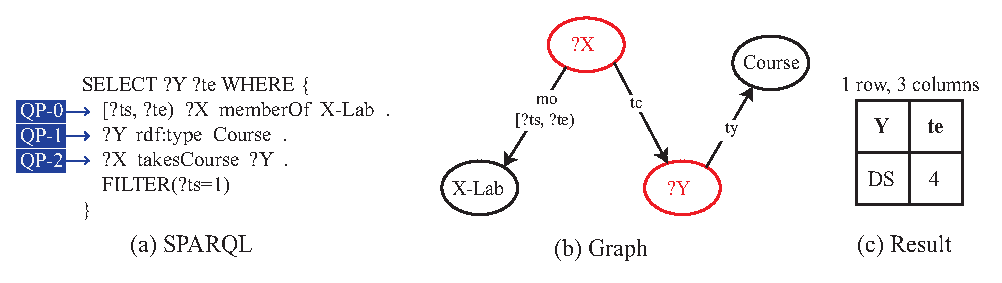
\includegraphics[width=0.9\textwidth]  {figures/tsparql.eps}} 
\bicaption{示例时序RDF图上的一条SPARQL-T查询语句}{A SPARQL-T query statement on the temporal RDF graph example}
\label{tsparql}
\end{figure}

图\ref{tsparql}给出了一条图\ref{trdf}中的时序RDF图上的SPARQL-T语句示例。
QP-0包含两个时间变量\texttt{ts}和\texttt{te},它们应该分别取值为匹配到的时序三元组的有效时间区间的开始时间和截止时间。
GP还包含一个过滤器,它会过滤出变量\texttt{ts}的取值为1的查询结果条目。
GP中的三个模式构成了图\ref{tsparql}(b)所示的查询图,可以在图\ref{trdf}中的时序RDF图上找到一个与之匹配的子图,
过滤后得到的查询结果如图\ref{tsparql}(c)所示,共一行二列。

\subsection{时序超图查询语言HQL-T}
时序超图是一种表示集合关系的数据模型,所以时序超图查询语言应该着重查询\textbf{集合间的关系}(即时序超边间的关系)、\textbf{元素和集合间的关系}(即顶点和时序超边间的关系)以及\textbf{元素间的关系}(即顶点间的关系)。此外,时序超图查询语言也应当支持\textbf{对时序超边的有效时间的查询}以及\textbf{基于有效时间的筛选}。

HQL-T查询语句的基础形式依然是
\begin{equation}
    \mathtt{SELECT \ RD \ WHERE \ GP}
\end{equation}
其中GP由一组基础关系模式(RP)组成,也可以包含过滤器,过滤器和RD的作用与SPARQL-T中的相同。给定一个时序超图$G$和一个HQL-T查询语句$Q$,HQL-T执行引擎会根据GP指定的模式在$G$中搜索与之匹配的子结构,找到RD中所有变量的可取值。RP的基本结构为:
\begin{equation}
    \mathtt{input \ builtin\colon \! type(args) \ output \ interval}
\end{equation}
其中\texttt{input}是输入元素列表,\texttt{builtin}是内置关键字,\texttt{type}指定了该模式的类型,\texttt{args}是该模式的参数,\texttt{output}是输出元素列表。\texttt{interval}是可选的,它是一个由两个变量组成的区间,格式为\texttt{[?var$_1$,?var$_2$)},当它出现在RP中时,HQL-T执行引擎应当将变量\texttt{var$_1$}和\texttt{var$_2$}分别取值为使得此RP成立的时间区间的开始时间和截止时间。
根据\texttt{type}的值,RP可分为以下几类:

\begin{figure}[!htb]
\center{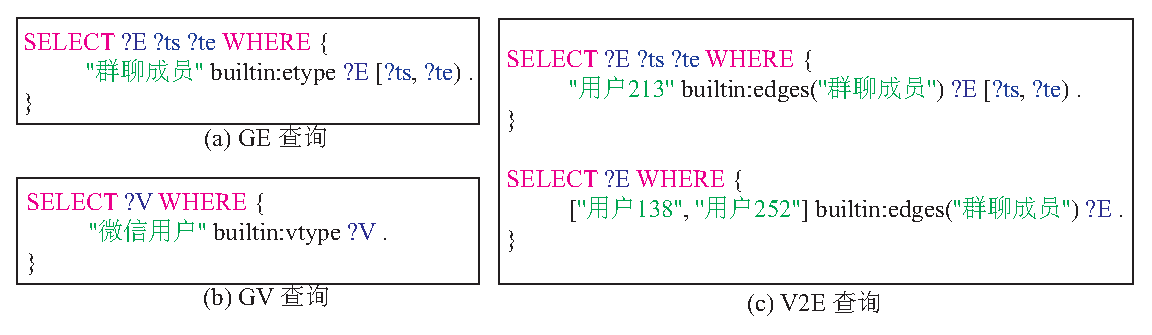
\includegraphics[width=0.9\textwidth]  {figures/hqls1.eps}} 
\bicaption{HQL-T查询语句示例(1)}{HQL-T query statement example (1)}
\label{hql1}
\end{figure}

\begin{itemize}
\item \textbf{GE模式:}该类型RP的\texttt{type}为\texttt{etype},输入元素列表要求只包含一个表示时序超边类型的常量;输出元素列表要求只包含一个变量;没有参数。这类RP的作用是查询所有指定类型的时序超边。如果包含\texttt{interval},那么变量\texttt{var$_1$}和\texttt{var$_2$}会分别取值为查询到的时序超边的有效时间区间的开始时间和截止时间。图\ref{hql1}(a)给出了一条只包含GE模式的HQL-T查询语句示例,该查询是要查找所有类型为“群聊成员”的时序超边。
\item \textbf{GV模式:}该类型RP的\texttt{type}为\texttt{vtype},输入元素列表要求只包含一个表示顶点类型的常量;输出元素列表要求只包含一个变量;没有参数。这类RP的作用是查询所有指定类型的顶点。由于顶点没有时序数据,所以\texttt{interval}不能出现在这类RP中。图\ref{hql1}(b)给出了一条只包含GV模式的HQL-T查询语句示例,该查询是要查找所有类型为“微信用户”的顶点。
\item \textbf{V2E模式:}该类型RP的\texttt{type}为\texttt{edges},输入元素列表可以包含若干表示顶点的常量或变量,输出元素列表要求只包含一个表示时序超边的变量,参数必须是一个表示时序超边类型的常量。这类RP的作用是查找所有指定类型且同时包含各输入顶点的时序超边。如果包含\texttt{interval},那么变量\texttt{var$_1$}和\texttt{var$_2$}会分别取值为查询到的时序超边的有效时间区间的开始时间和截止时间。图\ref{hql1}(c)给出了两条只包含V2E模式的HQL-T查询语句示例,第一个查询是要查找所有类型为“群聊成员”且包含顶点“用户213”的时序超边,第二个查询是要查找所有类型为“群聊成员”且同时包含顶点“用户138”和“用户252”的时序超边。
\end{itemize}

\begin{figure}[!htb]
\center{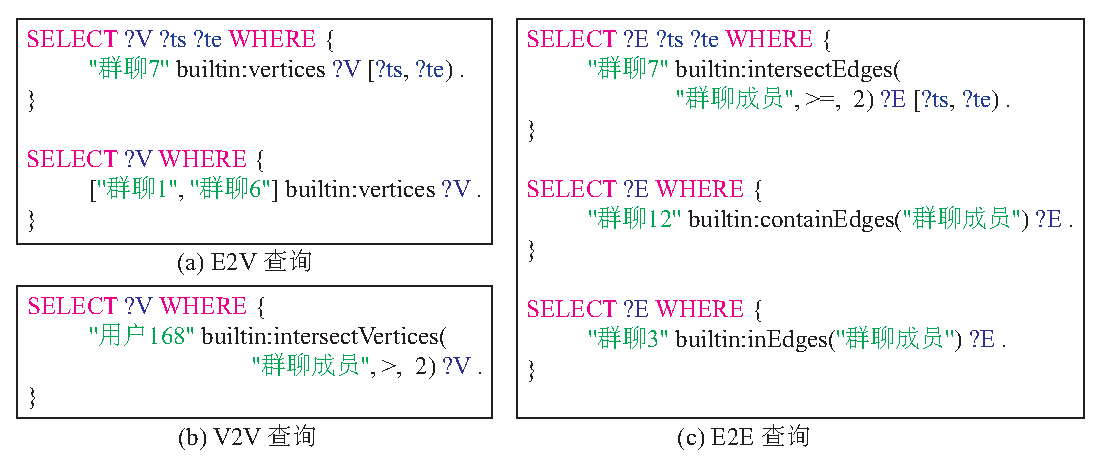
\includegraphics[width=0.9\textwidth]  {figures/hqls2.eps}} 
\bicaption{HQL-T查询语句示例(2)}{HQL-T query statement example (2)}
\label{hql2}
\end{figure}

\begin{itemize}
\item \textbf{E2V模式:}该类型RP的\texttt{type}为\texttt{vertices},输入元素列表可以包含若干表示时序超边的常量或变量,输出元素要求只包含一个表示顶点的变量,没有参数。这类RP的作用是查找各输入时序超边包含的所有公共顶点。如果包含\texttt{interval},那么变量\texttt{var$_1$}和\texttt{var$_2$}会分别取值为能够使得各输入时序超边都有效的最大时间区间的开始时间和截止时间。图\ref{hql2}(a)给出了两条只包含E2V模式的HQL-T查询语句示例,第一个查询是要查找时序超边“群聊7”的有效时间区间和包含的所有顶点,第二个查询是要查找时序超边“群聊1”和“群聊6”包含的公共顶点。
\item \textbf{V2V模式:}该类型RP的\texttt{type}为\texttt{intersectVertices},输入元素列表可以包含若干表示顶点的常量或变量,输出元素要求只包含一个表示顶点的变量。要求有三个参数,第一个参数是时序超边的类型,第二个参数是比较运算符,可以是$>$、$<$、$=$、$!=$、$>=$和$<=$其中之一,该参数可以省略,省略时默认是$>=$,第三个参数是一个整数。这类RP的作用是查找同时与各输入顶点出现在相同时序超边的顶点,且时序超边的类型和数量要满足参数的要求。这类RP不能包含\texttt{interval}。图\ref{hql2}(b)给出了一条只包含V2V模式的HQL-T查询语句示例,该查询是要查找与顶点“用户168”同时加入超过2个共同群聊的顶点。
\item \textbf{E2E模式:}该类型RP的\texttt{type}为\texttt{intersectEdges}、\texttt{containEdges}或\texttt{inEdges},输入元素列表可以包含若干表示时序超边的常量或变量,输出元素要求只包含一个表示时序超边的变量。当\texttt{type}为\texttt{intersectEdges}时,要求有三个参数,第一个参数是时序超边的类型,第二个参数是比较运算符,可以是$>$、$<$、$=$、$!=$、$>=$和$<=$其中之一,该参数可以省略,省略时默认是$>=$,第三个参数是一个整数,这类RP的作用是查找与各输入时序超边的交集的基数满足参数要求的时序超边;当\texttt{type}为\texttt{containEdges}或\texttt{inEdges}时,参数必须是一个表示时序超边类型的常量,这类RP的作用是查找指定类型且是各输入时序超边子集(当\texttt{type}为\texttt{containEdges}时)或超集(当\texttt{type}为\texttt{inEdges}时)的时序超边。如果包含\texttt{interval},那么变量\texttt{var$_1$}和\texttt{var$_2$}会分别
取值为能够使得各输入、输出时序超边同时有效的最大时间区间的开始时间和截止时间。图\ref{hql2}(c)给出了三个只包含E2E模式的HQL-T查询语句示例,第一个查询是要查找与时序超边“群聊7”拥有不少于2个公共顶点的类型为“群聊成员”的时序超边,第二个查询是要查找所有顶点都在时序超边“群聊12”中且类型为“群聊成员”的时序超边,第三个查询是要查找包含时序超边“群聊3”的所有顶点且类型为“群聊成员”的时序超边。
\end{itemize}

以上六类RP的组合可以实现很强的查询语义,基本可以满足对时序超图的查询需求。对于包含多RP的HQL-T查询语句,查询引擎需要按序逐条执行各RP。图\ref{hql}是一条包含两个RP的查询语句,在执行该语句时,需要先找到所有类型为“群聊成员”的时序超边,然后将找到的所有时序超边依次作为输入元素,查找其包含的所有顶点,最后过滤出符合条件的查询结果。

\begin{figure}[!htb]
\center{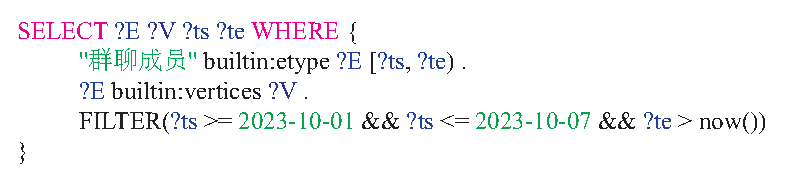
\includegraphics[width=0.8\textwidth]  {figures/hql.eps}}
\bicaption{普通HQL-T查询语句示例}{Common HQL-T query statement example}
\label{hql}
\end{figure}